%; whizzy chapter
% -initex iniptex -latex platex -format platex -bibtex jbibtex -fmt fmt
% 以上 whizzytex を使用する場合の設定。


%     Tokyo Debian Meeting resources
%     Copyright (C) 2008 Junichi Uekawa

%     This program is free software; you can redistribute it and/or modify
%     it under the terms of the GNU General Public License as published by
%     the Free Software Foundation; either version 2 of the License, or
%     (at your option) any later version.

%     This program is distributed in the hope that it will be useful,
%     but WITHOUT ANY WARRANTY; without even the implied warranty of
%     MERCHANTABILITY or FITNESS FOR A PARTICULAR PURPOSE.  See the
%     GNU General Public License for more details.

%     You should have received a copy of the GNU General Public License
%     along with this program; if not, write to the Free Software
%     Foundation, Inc., 51 Franklin St, Fifth Floor, Boston, MA  02110-1301 USA

%  preview (shell-command (concat "evince " (replace-regexp-in-string "tex$" "pdf"(buffer-file-name)) "&"))
% 画像ファイルを処理するためにはebbを利用してboundingboxを作成。
%(shell-command "cd image200804; ebb *.png")

%%ここからヘッダ開始。

\documentclass[mingoth,a4paper]{jsarticle}
\usepackage{monthlyreport}

% 日付を定義する、毎月変わります。
\newcommand{\debmtgyear}{2008}
\newcommand{\debmtgmonth}{5}
\newcommand{\debmtgdate}{15}
\newcommand{\debmtgnumber}{40}

\begin{document}

\begin{titlepage}
\thispagestyle{empty}

% タイトルページ:編集必要な部分は最初のマクロに飛ばすこと

\vspace*{-2cm}
第\debmtgnumber{}回 東京エリア Debian 勉強会資料

\hspace*{-2.4cm}
\includegraphics[width=210mm]{image200801/2008title.eps}\\
\hfill{}\debmtgyear{}年\debmtgmonth{}月\debmtgdate{}日

\end{titlepage}

\dancersection{Introduction}{上川 純一}
 
 今月のDebian勉強会へようこそ。これからDebianの世界にあしを踏み入れると
 いう方も、すでにどっぷりとつかっているという方も、月に一回Debianについ
 て語りませんか?

 Debian勉強会の目的は下記です。

\begin{itemize}
 \item \underline{Debian Developer} (開発者)の育成。
 \item 日本語での「\underline{開発に関する情報}」を整理してまとめ、アップデートする。
 \item \underline{場}の提供。
 \begin{itemize}
  \item 普段ばらばらな場所にいる人々が face-to-face で出会える場を提供
	する。
  \item Debian のためになることを語る場を提供する。
  \item Debian について語る場を提供する。
 \end{itemize}
\end{itemize}		

 Debianの勉強会ということで究極的には参加者全員がDebian Packageをがりがり
 と作るスーパーハッカーになった姿を妄想しています。情報の共有・活用を通し
 て Debianの今後の能動的な展開への土台として、「場」としての空間を提供す
 るのが目的です。

以上を目的とした、2008 年アジェンダです:
\begin{enumerate}
 \item 新年会「気合を入れる」
 \item Open Source Conference Tokyo (3/1)
 \item データだけのパッケージを作成してみる、
       ライセンスの考え方 (David Smith)
 \item バイナリ一つのパッケージを作成してみる (吉田@板橋)\\
       バージョン管理ツールを使いDebianパッケージを管理する(git)\\
       アップストリームの扱い(svn/git/cvs)(岩松 信洋さん)
 \item バイナリの分けたパッケージの作成。(前田さん)\\
       バイナリの分け方の考え方、アップグレードなどの運用とか。
 \item パッケージ作成(dpatch/debhelperで作成するパッケージ)(小林儀匡さん)\\
       man の書き方(roff or docbook)(でんさん)
 \item パッケージ作成(kernel patch、kernel module)
       、Debconf発表練習
 \item Debconf アルゼンチン、共有ライブラリパッケージ作成

 \item Open Source Conference Tokyo/Fall、
       デーモン系のパッケージの作成、latex、 emacs-lisp、フォントパッケージ
 \item パッケージの cross-compile の方法、amd64 上で i386 のパッケージと
       か、OSC-Fall報告会、Debconf報告会
 \item 国際化 po-debconf / po化 / DDTP
 \item 忘年会
\end{enumerate}


\newpage

\begin{minipage}[b]{0.2\hsize}
 \definecolor{titleback}{gray}{0.9}
 \colorbox{titleback}{\rotatebox{90}{\fontsize{80}{80} {\gt デビアン勉強会} }}
\end{minipage}
\begin{minipage}[b]{0.8\hsize}
\hrule
\vspace{2mm}
\hrule
\tableofcontents
\vspace{2mm}
\hrule
\end{minipage}

\dancersection{事前課題}{上川 純一}

今回の事前課題は以下です。

\begin{enumerate}
 \item 「フリーになって嬉しい/なると嬉しいソフトウェア」
 \item 「パッケージになって嬉しい/なると嬉しい/するのは難しそうなソフ
       トウェア」
 \item 「僕がゴールデンウィークに自由なソフトウェアのために行ったこと」
\end{enumerate}

この課題に対して提出いただいた内容は以下です。
\begin{multicols}{2}
\subsection{前田 耕平}

「フリーになって嬉しい/なると嬉しいソフトウェア」

djbdnsです。qmailははっきり言ってどうでも良いのですが、djbdnsは重宝してます。設定が簡単なのと、OpenBlockSでBINDを動かすのは重すぎるので軽快なdjbdnsとdnscacheは無いと困るので、今まではOBS用のコンパイル環境として古いiBookでビルドしてからOBSに流し込んでました。サーバにコンパイラを入れるのはナンセンスなので。

「パッケージになって嬉しい/なると嬉しい/するのは難しそうなソフトウェア」

Hobbit。これもこれでOBS用にビルドしないで済むようになったので。

「僕がゴールデンウィークに自由なソフトウェアのために行ったこと」

GWは子供の日が誕生日の嫁への奉仕が70%、家事が25%、今回の発表用の資料の下書き作成に5%でした。
\subsection{岩松 信洋}

「フリーになって嬉しい/なると嬉しいソフトウェア」
\begin{itemize}
 \item   Flash plugin\\
 先日 Flash に関するライセンスの変更がありましたけど、開発が
 少しは楽になるのかな、と思います。
\end{itemize}

「僕がゴールデンウィークに自由なソフトウェアのために行ったこと」

\begin{itemize}
 \item   Macbook iSight のファームウェアハック
 \item  Backlight をコントロールするための Xfce4 プラグインの開発
 \item  Xradnr を設定するための GUI開発 および Xfce4 プラグインの開発
 \item  Xfce の翻訳
 \item  U-boot for SuperH の開発
 \item  Debian kenrel module auto builder の妄想
 \item  Debian/SH の開発
\end{itemize}


\subsection{堀内寛己}

僕は無職の精神病者で、障害年金で暮らしています。
それで、毎日日曜プログラミングをしています。
自由なソフトウェアの作者として、ある意味究極の境遇にあるのかもしれません。

「僕がゴールデンウィークに自由なソフトウェアのために行ったこと」

ですから、ゴールデンウィークだからといって普段と差があるわけではありません。
たまたまこの時期、そして今も取り組んでいるのは、
レスキューOS作成用の、live-helperより気の利いたスクリプトの開発です。

このレスキューOSのファイルシステムは、USBフラッシュかNFSに置き、
必要なとき「だけ」CDに、ブートローダー「だけ」を置きます。

どうもlive-helperは、こういう用途に向いていないように思います。
live-helperの構成パラメータは山ほどありますが、これは
山ほど構成して1枚に焼きこんで、試してだめなら構成しなおし焼き直し、
という使い方を想定しているからに思えます。
僕が目指しているのはそういうものではありません。

live-helperの開発者は、LiveCD作りの発想から抜け出せないようです。
誤解があったら指摘してください。


\subsection{やまねひでき}

「フリーになって嬉しい/なると嬉しいソフトウェア」

\begin{itemize}
 \item adobe-cmap - これでハマることが多すぎです。
\end{itemize}

「パッケージになって嬉しい/なると嬉しい/するのは難しそうなソフトウェア」
 パッケージにした/しようとして止まっているのとかはあります。

\begin{itemize}
 \item  mirmon	-- ミラーサーバの状態チェックができます。スポンサー待ちで半年以上…
 \item  gnview	-- gtk2-perl の 2ch ブラウザ。スポンサー待ちです。
 \item  FailSafeC  -- 安全なC言語コンパイラ。upstream の man 作成やライセンスの確認待ち
 \item  naist-jdic -- non-free な ipadic の置き換え。upstream の作業待ち。
\end{itemize}

「僕がゴールデンウィークに自由なソフトウェアのために行ったこと」

ゴールデンウィークって何?だったので…
まぁ、いつも通りにパッケージのアップデートとかでした。
あ、そうそうミラーサーバの復旧作業してきました。機材は Ubuntu Japanese Team の方
から提供いただき、増設HDDは自費購入。

\subsection{吉田@板橋}

僕がゴールデンウィークに自由なソフトウェアのために行ったこと

ゴールデンウィーク(GW)には家のサーバのファイル名等のエンコーディングを
eucJPからUTF-8に変更する作業を行っていました。
そろそろ変えておいた方が、他の環境(今時のディストリービューションや
Windows等)との相互運用性が良いと判断し、時間がとれるGWに作業しました。
基本的にサービスを絞ったサーバ運用だったので、ファイル名変更のほかはsamba
やapache、bash等の設定変更のみでいけました。
その準備(バックアップ)として、漢字ファイル名を使用しているファイルに対
してkakasiおよびハードリンクを使用してローマ字にリネームするスクリプトを
(似たようなことをしているwebの記述を参考に)作成し、適用しました。
そのログやスクリプトはwebにある自分の備忘録に上げておきました、ご参考ま
で。


\subsection{あけど}

お題: パッケージになって嬉しい/なると嬉しい/するのは難しそうなソフトウェア

 実は「フリーになって嬉しい/なると嬉しいソフトウェア」ってのがあるのですが
たぶん他の方が触れられるかと思いますので、一つだけ挙げておきます。

adobe-cmap

これって元ネタはRFCらしいのですが、どうなったんでしょう?

 では本題、パッケージになって嬉しいというか「こんなのあったらなぁ」というのを挙げてみます。
テキストコンソールで日本語を扱っていると文字化けする事がよくあるのですが、
ターミナルの設定に合わせてコンソールのロケール情報を自動設定してくれる仕組みって欲しかったりします。(実はあったりします?)
termcap/terminfoの端末特性みたいな感じでフィルタを設定する仕組みとかどうかなぁ?
と思ってみたりしてます。

 もう一つ、以前挙げた iptables のフィルタですが、だれかパッケージにしてたりしませんか?
というか、自分で作ってみたら良いのかな?

\subsection{福永}

「僕がゴールデンウィークに自由なソフトウェアのために行ったこと」

現在、フリーのCommon Lispで並列計算を支援するライブラリは少ないので、
Common Lispで手軽に並列計算を出来る為にMPI並列プログラミングライブラリのForeign Function Interface
Library (言語バインディング)を作り始めました。基本的な通信Primitive(blocking/nonblocking,
system/self buffered)等のWrapper実装を終了し、任意のLispコードをSend/Receiveにより他CPUで実行出来るようになりました。
UFFIというポータブルなバインディングジェネレーターを用いたので、どのCommon Lisp実装でも使えるはずです。
今夏中、パッケージ化してリリースしたいと思います。

\subsection{奥野}

「フリーになると嬉しいソフトウェア」

Adobeのプラットフォーム(AIRとかFlashとかFlexとか)ですね。
Flashがないと見られないサイトが増えましたし、
AIRとかFlexとか一部ですげーとか言われてますが、
プロプライエタリなので普及すればするほどDebianのフリー的には面白くないのでは。

\subsection{沖中 研心}

「パッケージになると嬉しいソフトウェア」

商用のソフトウェア全般ですね。最近 Atok の deb パッケージが用意されていたりして、うれしく思うことがあります。
まだまだ Debian サポートしている商用ソフトウェアはほとんどないので、増えてくれるとうれしいですね。
個人的には、 トレンドマイクロの Internet Message Security Suite は、RedHat には対応していますが、
Debian には対応していないので、何とかなればいいのになぁと思ってます。

\subsection{日比野 啓}

表題: パッケージになって嬉しい/なると嬉しい/するのは難しそうなソフトウェア

Objective Camlを改造したものでMetaOCamlという実装(\url{http://www.metaocaml.org/})があるのですが、
これを使うと、LispのようなメタプログラミングをOCamlの型推論システムの上で
行なうことができるようになります。
すると、メタプログラミングで生成したOCamlプログラムを型推論で型付けすることができて、
型安全なメタプログラミングが行なえます。
パッケージにも是非してみたいのですが、すでにあるOCaml処理系とのインストール位置の棲み分けや
ライブラリのパッケージングが面倒そうです。

\subsection{山本 浩之}

「フリーになって嬉しい/なると嬉しいソフトウェア」

VMware が DFSG フリーになってくれるとかなり嬉しいです。あと悪名名高き Flash Player とか。
CMap は早くフリーになってくれると良いのですが…。
フリーになったといえば djb ソフトウェアがありますが、私自身はあまり恩恵を受けていません。

「パッケージになって嬉しい/なると嬉しい/するのは難しそうなソフトウェア」

パッケージにするのは難しいというより、安定版としてリリースされるものに取り込むのが難しそうなソフトウェアなら、youtube-dl とか
nicovideo-dl とか、あと 2ch ブラウザ類とかですかね?度々の仕様変更で全く使えなくなることもありますし。

「僕がゴールデンウィークに自由なソフトウェアのために行ったこと」

ITP をゴールデンウィーク中にできれば良かったのですが、できませんでした。スミマセン。
結局、今日のために、Debian GNU/Hurd いじりと、それを動かす環境作りで時間がなくなりました。


\subsection{野村 健太郎}
フリーになると嬉しいソフトウェア

Microsoft Office。金銭的・仕様的面からフリーになって欲しいという意味で。
Office 文書がプラットフォームに関係なく使用可能になれば、PC から Windows
完全消去の実現に一歩近づく。XPまでは仕方なく使っていたが、Vistaで我慢の
限界。ノートPCにプリインストールされている Vista(最低20Gは必要) のおかげで、
デュアルブートの Debian 用に思いっきりディスクを割けない。先月、Office 2007
の文書フォーマットである Open XML がISOの標準として承認されたそうだが、GPL
とは相容れないという情報もあり、どうなるのやら。

\subsection{藤沢 理聡}

「フリーになって嬉しい/なると嬉しいソフトウェア」
 「自由」という意味のフリーだとちょっと思いつかないので、「無償」の意味の
方であげるなら、Operaブラウザです。様々なOSに対応しているWebブラウザの中で
私の周囲で最も利用されているのはFirefoxですが、私自身はOpera派なので、Opera
が無償になったときは喜びました。Debianしか使わないなら特にOperaにこだわりま
せんが、他のOSも頻繁に利用する環境では、できれば利用する全てのOSに対応して
いることが望ましいと思っています。

\subsection{荒木 靖宏}

「僕がゴールデンウィークに自由なソフトウェアのために行ったこと」

ちょうどGWは出張だったのですが、出張で成田に行く途中でメンテをしているsip-testerにstrcatつかってんぞ、strncatのつかいかたが間違っているぞ、というdebian
security teamからのBTSがやってきました。そのおかげでしばしたのしい思いをしながらヒコーキにのりこみ、出張先についてこちらからメールを出したら即パッチがやってきました。
というわけで自分がやったことといえば、それをupstreamに伝えるだけ。upstreamにmailをしたらupstreamは休暇中だよーというメールが戻ってきたのでした。

「フリーになって嬉しい/なると嬉しいソフトウェア」

自分が仕事で書いたコードですね。railsで書いているだけに公開したいしたい。

\end{multicols}

%%% trivia quiz
\dancersection{Debian Trivia Quiz}{小林 儀匡}

ところで、みなさん Debian 関連の話題においついていますか?Debian関連の話
題はメーリングリストをよんでいると追跡できます。ただよんでいるだけではは
りあいがないので、理解度のテストをします。特に一人だけでは意味がわからな
いところもあるかも知れません。みんなで一緒に読んでみましょう。

今回の出題範囲は\url{debian-devel-announce@lists.debian.org} に投稿された
内容とDebian Project Newsからです。
% 出題範囲: http://lists.debian.org/debian-devel-announce/2008/04/msg00010.html 〜 http://lists.debian.org/debian-devel-announce/2008/05/msg00003.html
\begin{multicols}{2}
 
 \subsection{debian-devel-announce}
 \url{debian-devel-announce@lists.debian.org}への投稿内容からです。
 
 \santaku
 {Joerg Jaspertがdakのソースコードに取り込んだ、Thomas Viehmannからのパッチとは?}
 {パッケージを受け取ったときにメンテナだけでなくスポンサーにもメールを送るようにするパッチ}
 {パッケージを受け取ったときに現在のカルマをメンテナに通知するパッチ}
 {パッケージを受け取ったときに現在のバグの一覧をメンテナに通知するパッチ}
 {A}
 
 \santaku
 {debhelperバージョン7では、何から学んだことを取り込んでいるか}
 {MSDN}
 {CDDB}
 {CDBS}
 {C}
 
 \santaku
 {新たにリリースマネージャになったのは?}
 {Andreas Barth}
 {Luk Claes}
 {Marc 'HE' Brockschmidt}
 {C}
 
 \santaku
 {Debianパッケージメンテナンスに関する自動通知メールにおいて、メールを生成したソフトウェアを示すのに使うよう提案されたメールヘッダは?}
 {X-Debian:}
 {X-Debian-Package:}
 {User-Agent:}
 {A}
 
 \subsection{2008年01号}
 \url{http://www.debian.org/News/weekly/2008/01/}
 にある4月21日版です。
 
 \santaku
 {Siobh\'an O'MahonyとFabrizio Ferraroの研究ではDebianの統治システムの歴史を4つの時期に分けているが、そのうち1999年から2003年に当たるものは?}
 {Stabilizing Governance}% 2003-2006
 {Implementing Governance}% 1999-2003
 {Designing Governance}% 1997-1999
 {B}
 
 \santaku
 {Institute for Advanced Professional Studies Yankee groupの研究結果として適切でないものは?}
 {2006年と比べてDebianサーバのダウンタイムが41\%{}減った}
 {2006年と比べてネットワークに1台以上のDebianを入れているユーザが15\%{}から24\%{}に上昇した}
 {2006年と比べてDebianユーザが41\%{}減った}
 {C}
 
 \santaku
 {開発者のブログ記事を収集して表示するPlanet Debianに関して、Martin Joey Schulzeが始めたサービスとは?}
 {記事をメーリングリストとして購読できるようにするサービス}
 {すべての記事に対してコメントを一斉に送れるようにするサービス}
 {記事をSlashdotや各種ソーシャルブックマークサービスに容易に投稿できるようにするサービス}
 {A}
 
 \santaku
 {Christian Perrierによると、最近正式なDebian開発者として登録されたメンバーの女性率は?}
 {5\%{}}
 {10\%{}}
 {50\%{}}
 {B}
 
 \subsection{2008年02号}
 \url{http://www.debian.org/News/weekly/2008/02/}
 にある5月9日版です。
 
 \santaku
 {WWWの生みの親として有名なTim Berners-LeeがWWW2008カンファレンスの基調演説でDebianについて述べたこととは?}
 {Debianのウェブページのように古臭いページは消えていく運命にある}
 {Debianのウェブページは様々な言語に地域化されており素晴らしい}
 {Debianのパッケージングシステムは素晴らしい}
 {C}
 
 \santaku
 {今年のGoogle Summer of CodeプログラムでDebian Projectのタスクを得た学生の人数は?}
 {6}
 {12}
 {24}
 {B}
 
 \santaku
 {5月9日現在、lennyのリリースに向けて進められている移行の状況として適切でないものは?}
 {Perlのバージョン5.10をlennyでデフォルトとするための移行作業が行われている}
 {既にlennyにおいてPythonのデフォルトがバージョン2.5になっている}
 {Rubyのバージョン1.9をlennyでデフォルトとするための移行作業が行われている}
 {C}
 
 \santaku
 {4月18日に何人のDebian正式開発者が追加されたか?}
 {9}
 {19}
 {29}
 {B}
 
\end{multicols}

\dancersection{最近のDebian関連のミーティング報告}{上川 純一}
\subsection{東京エリアDebian勉強会39回目報告}

% (query-replace-regexp "<.*?>" "")
% (query-replace-regexp "^[	 ]\+" "")

東京エリアDebian勉強会報告。
4月の第39回東京エリアDebian勉強会を実施しました。

今回の参加者は
あけどさん、やまねさん、山本浩之さん、前田さん、沖中さん、岩松さん、吉田さん、
山本琢さん、本庄さん、濱野さん、日比野啓さん、jitsukataさん、キタハラさ
ん、藤沢理聡さん、でんさん、
吉藤さん、上川の17人でした。

まず、クイズを今回も実施しました。
今回も、debian-devel-announce の内容から出題しました。
今回の
景品はピンク色の「あれ」でした。

2008年のテーマはDEBパッケージの開発・管理に関連した内容ですが、
二回目のテーマとしてバイナリパッケージ一つの場合の話をしました。
吉田さんがdebhelper を使った流れを紹介しました。

岩松さんが Git を使った場合のDebian パッケージの管理方法について紹介しました。

上川が Nexenta Core Platform をインストールしてみて試した内容について報告しました。

今回は宴会は駒忠
にて開催しました。

\dancersection{バイナリをわけたパッケージの扱い}{前田 耕平}
\label{sec:multibinpkg}
\index{ふくすうばいなりのぱっけーじ@複数バイナリのパッケージ} 
\index{ぱっけーじ@パッケージ}

\subsection{はじめに}

今回はDebianパッケージを作成した経験がほぼ無い人を対象とし、先月
\footnote{2008年4月} の『バイナリ一つだけのパッケージを作成してみる』を
予習していることを前提とします。

一応、前回の内容もおさらいしながら、今回もdh\_makeを使って、debhelperス
タイルでの複数のバイナリに分けてパッケージを作る方法を説明しますので、前
回参加できなかったとしても、ある程度は問題ないかと思います。

\subsection{バイナリの分け方の考え方}
通常のパッケージは、一つのバイナリパッケージとして作成・配布されるケー
スが多いでしょう。ではどのようなケースにおいて、バイナリパッケージは複数
に分けられているのでしょうか。大きく分けると次の三パターンくらいになりそう
です。

\begin{itemize}
 \item
開発環境と実行環境

例)
      \begin{itemize}
       \item
	    JavaのSDKとJRE

      \end{itemize}
 \item
C/Sモデルのサーバ側プログラムとクライアント側プログラム

例)
      \begin{itemize}
       \item
	    bindとdnsutils
      \end{itemize}

 \item
プログラム本体とアドオンで追加可能なモジュール、ユーティリティ

例)
      \begin{itemize}
       \item
	    ApacheとApache moduleやApache Bench
      \end{itemize}
\end{itemize}

これらに共通して言えるのは、単一のソースツリーから複数に分けることにより、
導入するユーザの使い勝手が良くなる、ということだと言えると思います。

なお、複数のバイナリパッケージを作成するときも、ソースツリー及びソースパッ
ケージ自体は単一なので、複数のソースツリー・ソースパッケージから生成され
る事はありません。

\subsection{前回のおさらい}

前回は、dh\_makeを使って、debhelperスタイルで単一のバイナリパッケー
ジを作りました。今回は、まず簡単なCのプログラムとMakefileを用意して、それを
Debianパッケージにします。そこで単一のバイナリパッケージの場合と複数のバ
イナリパッケージに分ける場合との違いを見てみましょう。

\subsubsection{ソースコードとMakefileの用意}
 まず、下記のようなディレクトリ、ファイルを用意します。
 \begin{commandline}
hoge-1.0/
 hoge.c
 Makefile
 \end{commandline}
 ファイルはそれぞれ下記のようなコードを書きます。
 \begin{itemize}
  \item
       hoge.c
       \begin{commandline}
#include <stdio.h>
      
int main(void)
{
       printf(``hello\n'');
       return 0;
}
       \end{commandline}
  \item
       Makefile
       \begin{commandline}
CC=gcc
CFLAGS=-O
BINDIR=/usr/games
     
hoge: hoge.c
       $(CC) $(CFLAGS) -o hoge hoge.c
       
install:
       install -d ${DESTDIR}${BINDIR}
       install -m 755 hoge ${DESTDIR}${BINDIR}
       
clean:
       rm -f hoge
       \end{commandline}
 \end{itemize}

\subsubsection{dh\_makeでテンプレートの作成}
それでは、前回と同様にdh\_makeを使ってシングルパッケージを作ってみます。
まず、dh\_makeでテンプレートを作ります。

\begin{commandline}
$ cd hoge-1.0

$ dh_make --single -c gpl --createorig
Maintainer name : Kouhei Maeda
Email-Address   : mkouhei@gmail.com
Date            : Sat, 10 May 2008 15:36:29 +0900
Package Name    : hoge
Version         : 1.0
License         : gpl
Type of Package : Single
Hit <enter> to confirm: 
Done. Please edit the files in the debian/ subdirectory now. You should also
check that the hoge Makefiles install into $DESTDIR and not in / .
\end{commandline}

\subsubsection{debianディレクトリ以下のファイルの編集}

debianディレクトリ以下を編集します。
\begin{commandline}
$ cd debian

$ rm *ex *EX (<-不要なサンプルファイルを削除します。)
\end{commandline}

\begin{itemize}
 \item
      debian/control
      \begin{commandline}
Source: hoge
Section: games
Priority: extra
Maintainer: Kouhei Maeda <mkouhei@gmail.com>
Build-Depends: debhelper (>= 5)
Standards-Version: 3.7.2

Package: hoge
Architecture: any
Depends: ${shlibs:Depends}, ${misc:Depends}
Description: sample program
 Hello hoge program
      \end{commandline}
 \item
      debian/copyright
      \begin{commandline}
This package was debianized by Kouhei Maeda <mkouhei@gmail.com> on
Sat, 10 May 2008 15:36:29 +0900.

It was downloaded from <http://www.palmtb.net>

Upstream Author(s):

    <Kouhei Maeda mkouhei@gmail.com>

Copyright: 

    <Copyright (C) 2008 Kouhei Maeda>

License:
(以下、省略) 
      \end{commandline}

 \item
      debian/dirs\footnote{hogeのインストール先を指定します。}
      \begin{commandline}
usr/games
      \end{commandline}

 \item
      debian/changelog
      \begin{commandline}
$ dch
hoge (1.0-1) unstable: urgency=low

  * Initial release

 -- Kouhei Maeda <mkouhei@gmail.com>  Sat, 10 May 2008 15:47:41 +0900
      \end{commandline}
\end{itemize}

\subsubsection{パッケージ作成}
それでは、debuildコマンドでパッケージを作成してみます。
\begin{commandline}
$ debuild -us -uc
\end{commandline}

debファイルができているのを確認します。
\begin{commandline}
$ cd ../../
$ ls hoge_1.0*
hoge_1.0-1.diff.gz  hoge_1.0-1_i386.build    hoge_1.0-1_i386.deb
hoge_1.0-1.dsc      hoge_1.0-1_i386.changes  hoge_1.0.orig.tar.gz
\end{commandline}

上記のような簡単なものであれば、rulesファイルを修正しなくても、パッケー
ジを作れる事が分かります。ちゃんとやるには、lintianのエラーや警告を潰し、
pbuilderでのチェックやインストール、アンインストールのチェックをする必要
がありますが、ここでは省略します。

\subsection{複数のバイナリパッケージを作ってみる。}
それでは、今度は先ほどの簡単なコードを一部変更して、それぞれ別のパッケー
ジになるようにします。

\subsubsection{ソースコード、Makefileの用意}
下記のようなファイルを用意します。先ほどのhoge-1.0をコピーして修正すれば
よいでしょう。

\begin{commandline}
foo-1.0/
 foo.c
 bar.c
 Makefile
\end{commandline}
各ファイルは下記のようにします。
\begin{itemize}
 \item
      foo.c
      \begin{commandline}
#include <stdio.h>

int main(void)
{
  printf(``hello,foo\n'');
  return 0;
}
      \end{commandline}
 \item
      bar.c
      \begin{commandline}
#include <stdio.h>

int main(void)
{
  printf(``hello,bar\n'');
  return 0;
}
      \end{commandline}
 \item
      Makefile
      \begin{commandline}
CC=gcc
CFLAGS=-O
BINDIR=/usr/games

foo:
       $(CC) $(CFLAGS) -o foo foo.c
       $(CC) $(CFLAGS) -o bar bar.c

install:
       install -d ${DESTDIR}${BINDIR}
       install -m 755 foo ${DESTDIR}${BINDIR}
       install -m 755 bar ${DESTDIR}${BINDIR}

clean:
       rm -f foo bar
      \end{commandline}
\end{itemize}
上記をmakeすると、fooとbarという実行ファイルができます。今回は、これらを
それぞれfooパッケージとbarパッケージの別々のパッケージにしてみます。

\subsubsection{dh\_makeの実行}
単一のバイナリパッケージとは違い、dh\_makeを実行するときのオプション
を''--single''から''--multi''に変更して実行します。

\begin{commandline}
$ cd foo-1.0
$ dh_make --multi -c gpl --createorig
Maintainer name : Kouhei Maeda
Email-Address   : mkouhei@gmail.com
Date            : Sat, 10 May 2008 16:32:38 +0900
Package Name    : foo
Version         : 1.0
License         : gpl
Type of Package : Multi-Binary
Hit <enter> to confirm: 
Done. Please edit the files in the debian/ subdirectory now. You should
 also
check that the foo Makefiles install into $DESTDIR and not in / .
\end{commandline}

単一のバイナリパッケージの時と同様に、debianディレクトリとその下にファイ
ルが作成されます。

単一のバイナリの時に比べ、以下のファイルが増えていることが分かります。
このテンプレートと同様なファイルが後ほどビルドする際に必要になります。
\begin{itemize}
 \item
      foo-doc.docs
 \item
      foo-doc.install
\end{itemize}

\subsubsection{debianディレクトリ以下のファイルの編集}
まず、単一のバイナリパッケージを作成するときと同じように修正して、ビル
ド出来るのか確認してみます。
最初に先ほどと同じように今回は必要のないサンプルファイルを削除します。

\begin{commandline}
$ cd debian
$ rm *ex *EX
\end{commandline}

次に、controlファイルを修正します。複数のバイナリパッケージを作成するに
は、空行で区切られた三つ以上のエントリが必要になります。

一つ目のエントリは、ソースパッケージ自身のことを記述するためのエントリで
す。二つ目以降のエントリが生成されるバイナリパッケージについての情報を記
述するエントリです。

今回は、fooとbarの二つのパッケージを作成するので、dh\_makeで作成されたテ
ンプレートを以下の様に変更します。

\begin{commandline}
Source: foo
Section: games (<- セクションを変更)
Priority: extra
Maintainer: Kouhei Maeda <mkouhei@gmail.com>
Build-Depends: debhelper (>= 5)
Standards-Version: 3.7.2

Package: foo
Architecture: any
Depends: ${shlibs:epends}, ${misc:Depends}
Description: sample program foo (<- 説明を記載)
 foo foo foo (<- 説明の詳細を記載)

Package: bar
Architecture: any (<- 今回はアーキテクチャ依存なのでanyにする)
Description: sample program bar (<- 説明を記載)
 bar bar bar (<- 説明の詳細を記載)
\end{commandline}

また、単一のバイナリパッケージの時と同様に、下記ファイルを修正します。
\begin{itemize}
 \item
      debian/copyright
 \item
      debian/changelog
 \item
      debian/dirs
\end{itemize}

修正後、シングルバイナリの時と同様にdebuildを実行してみます。
\begin{commandline}
$ debuild -us -uc
 dpkg-buildpackage -rfakeroot -D -us -uc
(中略)
dh_installdirs -s
# Add here commands to install the arch part of the package into 
# debian/tmp.
/usr/bin/make DESTDIR=/home/user/foo-1.0/debian/foo
 install
make[1]: ディレクトリ `/home/user/foo-1.0' に入ります
install -d /home/user/tmp/foo-1.0/debian/foo/usr/games
install -m 755 foo
 /home/user/foo-1.0/debian/foo/usr/games
install: cannot stat `foo': そのようなファイルやディレクトリはありません
make[1]: *** [install] エラー 1
make[1]: ディレクトリ `/home/user/foo-1.0' から出ます
make: *** [install-arch] エラー 2
dpkg-buildpackage: failure: fakeroot debian/rules binary gave error exit
 status 2
debuild: fatal error at line 1319:
dpkg-buildpackage -rfakeroot -D -us -uc failed
\end{commandline}

どうやら、単一のバイナリパッケージの時にはちゃんと作成されていた実行ファイ
ルが今回は作成されていない様です。単一のバイナリパッケージを作成する時は、
rulesファイルのbuild-stampターゲットの中で、\$(MAKE)コマンドが記述されて
いましたが、複数のバイナリパッケージの場合は、rulesファイルの中で、
\$(MAKE)がコメントアウトされており、デフォルトではmakeが実行されません。
そのため、rulesファイルを修正する必要があります。

{\bf ''--single''の時のrulesファイル}
\begin{commandline}
build: build-stamp

build-stamp: configure-stamp 
 dh_testdir

 # Add here commands to compile the package.
 $(MAKE)
 #docbook-to-man debian/hoge.sgml > hoge.1

 touch $@
\end{commandline}

\subsubsection{rulesの記述}
rulesの必須ターゲットは、単一のバイナリパッケージの時と同様に、build,
binary, binary-indep, binary-archの4つです。

'--multi'オプションで作成されるrulesではbuildターゲットは下記の様になっ
ています。
\begin{commandline}
build: build-arch build-indep

build-arch: build-arch-stamp

build-arch-stamp: configure-stamp

        # Add here commands to compile the arch part of the package.
        #$(MAKE)
        touch $@

build-indep: build-indep-stamp

build-indep-stamp: configure-stamp

        # Add here commands to compile the indep part of the package.
        #$(MAKE) doc
        touch $@
\end{commandline}

今回、fooもbarも、gccでコンパイルするので、controlファイルでの
Architectureセクションではどちらもanyを記述しています。そのため、今回は
rulesファイルでは、buildターゲットでは、build-arch、build-arch-stampに依
存しますが、build-arch-stampの中でコメントアウトされている\$(MAKE)を有
効にする必要があるので、有効にして、ビルドします。

\begin{commandline}
$ debuild -us -uc
 dpkg-buildpackage -rfakeroot -D -us -uc
(中略)
dpkg-buildpackage: full upload (original source is included)
Now running lintian...
(中略)
Finished running lintian.
\end{commandline}

今回は、うまくビルドできたように見えます。パッケージのビルド時には、
{\bf debian/パッケージ名}ディレクトリが作成され、そこにパッケージ含
まれるファイルがコピーされます。ですので、ちゃんと期待するファイルがコピー
されているのか確認してみます。

\begin{commandline}
$ tree debian/{foo,bar}
debian/foo
|-- DEBIAN
|   |-- control
|   `-- md5sums
`-- usr
    |-- bin
    |-- games
    |   |-- bar
    |   `-- foo
    |-- sbin
    `-- share
        `-- doc
            `-- foo
                |-- README.Debian
                |-- changelog.Debian.gz
                `-- copyright
debian/bar
|-- DEBIAN
|   |-- control
|   `-- md5sums
`-- usr
    `-- share
        `-- doc
            `-- bar
                |-- changelog.Debian.gz
                `-- copyright

13 directories, 11 files
\end{commandline}

実行ファイルfoo, barが今度はきちんと作成されていますが、barファイルは期
待するディレクトリbar/usr/games以下にコピーされていません。bar/usr/games
ディレクトリ自体も作成されていない事が分かります。
複数のバイナリパッケージを作成するには、rulesファイルを上記の変更だけで
なく、さらにもう一ヶ所修正し、さらに以下のファイルを作成する必要がありま
す。
\subsubsection{rulesファイルで修正が必要な箇所}
debian/rules
\begin{commandline}
build: build-arch build-indep

build-arch: build-arch-stamp
build-arch-stamp: configure-stamp

        # Add here commands to compile the arch part of the package.
        $(MAKE) (<-最初の変更箇所。)
        touch $@
(中略)
install-arch:
        dh_testdir
        dh_testroot
        dh_clean -k -s
        dh_installdirs -s

        # Add here commands to install the arch part of the package into
        # debian/tmp.
        $(MAKE) DESTDIR=$(CURDIR)/debian/tmp install (<-debian/fooを
 # debian/tmpに修正します。)

        dh_instll -s
\end{commandline}

\subsubsection{新規作成するファイル}
\begin{itemize}
 \item
      foo.install
      \begin{commandline}
debian/tmp/usr/games/foo
      \end{commandline}
 \item
      bar.install
      \begin{commandline}
debian/tmp/usr/games/bar
      \end{commandline}
\end{itemize}

複数のバイナリパッケージを作成する場合、ビルド時には、通常、ソフトウェア
のファイルやディレクトリを、まず{\bf debian/パッケージ名}ディレクトリ以外
の一時ディレクトリ\footnote{通常はdebian/tmpディレクトリなどを指定しま
す。} に仮インストールし、そこから{\bf debian/パッケージ名}ディレクトリに
コピーします。この時、dh\_installコマンドとdebianディレクトリ以下の{\bf
パッケージ名.install}ファイルが使用されます。


今回の場合、debian/foo.installファイルと、debian/bar.installファイルが使
われ、ここに記載したディレクトリやファイルが、それぞれのパッケージ用のディ
レクトリにコピーされます。

つまり、それぞれ以下のようにコピーされます。
\begin{itemize}
 \item
     foo.installに記載された''debian/tmp/usr/games/foo''ファイル

	   → パッケージfoo用にdebian/foo/usr/games/ディレクトリ以下に

 \item
      bar.installに記載された''debian/tmp/usr/games/bar''ファイル

      → パッケージbar用にdebian/bar/usr/games/ディレクトリ以下に

\end{itemize}

では、実際にビルドしてみます。
\begin{commandline}
$ debuild -us -uc
\end{commandline}

ビルドした結果の{\bf debian/パッケージ}ディレクトリと仮インストール用の
{\bf debian/tmp}ディレクトリを見てみましょう。
\begin{commandline}
$ tree tmp foo bar 
tmp
`-- usr
    `-- games
        |-- bar
        `-- foo
foo
|-- DEBIAN
|   |-- control
|   `-- md5sums
`-- usr
    |-- games
    |   `-- foo
    `-- share
        `-- doc
            `-- foo
                |-- README.Debian
                |-- changelog.Debian.gz
                `-- copyright
bar
|-- DEBIAN
|   |-- control
|   `-- md5sums
`-- usr
    |-- games
    |   `-- bar
    `-- share
        `-- doc
            `-- bar
                |-- changelog.Debian.gz
                `-- copyright

14 directories, 13 files
\end{commandline}
今度はちゃんとコピーされています。パッケージが作成されているか見てみます。
\begin{commandline}
$ cd ../../

$ ls foo_1.0* bar*
bar_1.0-1_i386.deb  foo_1.0-1_i386.build    foo_1.0.orig.tar.gz
foo_1.0-1.diff.gz   foo_1.0-1_i386.changes
foo_1.0-1.dsc       foo_1.0-1_i386.deb
\end{commandline}

pbuilderでチェック後、インストールしてみます。
\begin{commandline}
$ sudo dpkg -i foo_1.0-1_i386.deb
 bar_1.0-1_i386.deb 
未選択パッケージ foo を選択しています。
(データベースを読み込んでいます ... 現在 222038 個のファイルとディレクト
 リがインストールされています。)
(foo_1.0-1_i386.deb から) foo を展開しています...
未選択パッケージ bar を選択しています。
(bar_1.0-1_i386.deb から) bar を展開しています...
foo (1.0-1) を設定しています ...
bar (1.0-1) を設定しています ...
\end{commandline}

インストールできているか確認してみます。
\begin{commandline}
$ dpkg -L foo 
/.
/usr
/usr/share
/usr/share/doc
/usr/share/doc/foo
/usr/share/doc/foo/changelog.Debian.gz
/usr/share/doc/foo/README.Debian
/usr/share/doc/foo/copyright
/usr/games
/usr/games/foo

$ dpkg -L bar
/.
/usr
/usr/share
/usr/share/doc
/usr/share/doc/bar
/usr/share/doc/bar/changelog.Debian.gz
/usr/share/doc/bar/copyright
/usr/games
/usr/games/bar

$ dpkg -s foo bar
Package: foo
Status: install ok installed
Priority: extra
Section: games
Installed-Size: 44
Maintainer: Kouhei Maeda <mkouhei@gmail.com>
Architecture: i386
Version: 1.0-1
Depends: libc6 (>= 2.7-1)
Description: sample program foo
 foo foo foo

Package: bar
Status: install ok installed
Priority: extra
Section: games
Installed-Size: 40
Maintainer: Kouhei Maeda <mkouhei@gmail.com>
Architecture: i386
Source: foo
Version: 1.0-1
Description: sample program bar
 bar bar bar
\end{commandline}

\subsubsection{補足}
ちなみに、dh\_makeで''--multi''ではなく、''--single''を指定しても、ソー
スツリーのMakefileと、debian/rulesの記述を変更したところ、複数のバイナリ
パッケージに分ける事ができたので、結局はmake次第でどうにでもできるのでは
ないかと思います。

\subsection{まとめ}
前回を踏襲して、dh\_makeを使って、debhelperスタイルで複数のバイナリパッ
ケージを作ってみました。さらに、単一バイナリパッケージとの違いを分かりや
すくするため、非常に簡単なプログラムをパッケージにすることで、その違いを
見てみました。

単一バイナリパッケージを作成するときと同じような感覚でやると、rulesファ
イルのところで躓くので、パッケージの作成はmakefileを読めることが重要だと
いうことがよく実感できました。


\subsection{参考書籍}
\begin{itemize}
 \item
      入門 Debianパッケージ (ISBN:978-4-7741-2768-X)
 \item
      GNU Make 第3版 (ISBN:4-87311-269-9)
 \item
      第39会 東京エリアデビアン勉強会(2008年4月) 「バイナリ一つだけのパッ
      ケージを作成してみる」
 \item
      The Debian Systems その概念と技法 (ISBN:978-4-8399-1897-2)
\end{itemize}


\newpage

% ここからは月例特集。


%===========================================================%
\begin{getsureiupdate}{月例 Debian GNU/kFreeBSD}{大浦 真}
\index{kFreeBSD}
  Debian Project の大浦です。(現在、京都在住)
  今月からこの場をお借りして Debian GNU/kFreeBSDの状況をお伝えすることに
  なりました。
  よろしくお願いします。

  Debian は、現在、その OS の中心として Linux カーネルを利用していますが、
  Debian GNU/kFreeBSD とは、カーネルとして FreeBSD のカーネルを利用し、
  その上に GNU C library と GNU のユーザランド、および、
  Debian のパッケージセットを移植したものです。
  FreeBSD のカーネルだけを使っているので、``\textbf{k}FreeBSD'' と
  呼んでいます。

  そんな Debian GNU/kFreeBSD は、開発途上にあり、
  Debian の一部として、まだ、正式にはリリースされていません。
  しかし、FreeBSD のインストーラを改造した kFreeBSD 用のインストーラも
  用意されていますし、
  kFreeBSD 用の buildd も設置されていますので、
  比較的簡単に実機やエミュレータ上で試すことができます。
  また、X.Org も使えますので、それなりに使うことができるようになっています。
  ただ、重要なパッケージで、buildd でビルドできず、
  バイナリが用意されていないものがあったり、
  用意されていてもまともに動作しないものがあったりもするので、
  まだまだ、いろいろとハックのしがいがあると思います。

  Debian GNU/kFreeBSD に関する情報は、以下の Debian Wiki のページに
  まとまっていますので、
  ぜひご覧下さい。

  \url{http://wiki.debian.org/Debian%20GNU/kFreeBSD}
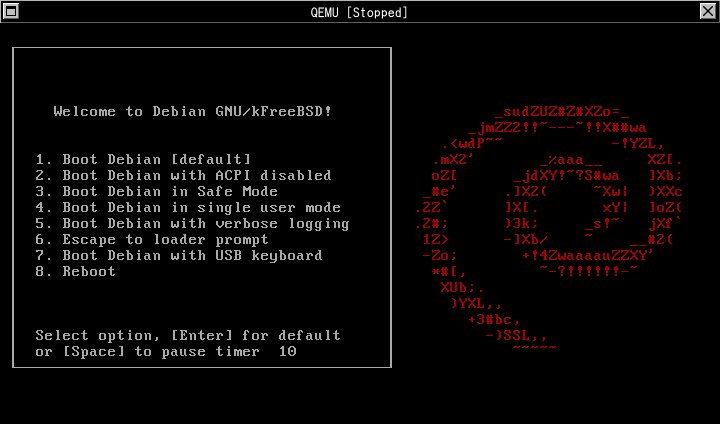
\includegraphics[width=1\hsize]{image200805/qemu-kfreebsd01.jpg}
\end{getsureiupdate}
%===========================================================%

%===========================================================%
\begin{getsureiupdate}{月例 Debian GNU/Linux SuperH port}{岩松 信洋}
\index{SuperH}
今月のDebian GNU/Linux SuperH 移植版の状況をお伝えします。

Debian/SH port は先月から加速しはじめました。
その理由として、フランス人の方が協力してくれることになったためです。
いまのところ、パッケージ用リポジトリを共同にしようということになっており、新しい
SH4用のリポジトリがフランスと日本にできました。

現在のステータスは、gcc-4.3 ベースでパッケージを作っています。
マシンが複数台あるのですが、builddをまだ1台しかセットアップしていません。
今月中には複数台セットアップしたいと考えています。

現在抱えている問題として、mesa のコンパイルに失敗するというものがありま
 す。
internal compiler error なので、調べるのは難しいですが、マクロ展開で
こけているところまで追いました。絶賛調査中です。

\begin{commandline}
gcc -c -I../../include -I../../src/mesa \
-I../../src/mesa/main \-I../../src/mesa/glapi \
-I../../src/mesa/math -I../../src/mesa/tnl 
-I../../src/mesa/shader \
-I../../src/mesa/shader/grammar \
-I../../src/mesa/shader/slang -I../../src/mesa/swrast \
-I../../src/mesa/swrast_setup -Wall -Wmissing-prototypes \
-O2 -g   -D_POSIX_SOURCE -D_POSIX_C_SOURCE=199309L \
-D_SVID_SOURCE -D_BSD_SOURCE -D_GNU_SOURCE -DPTHREADS\
 -DUSE_XSHM -DHAVE_POSIX_MEMALIGN  -I/usr/X11R6/include \
-std=c99 -ffast-math  -fno-strict-aliasing \
vbo/vbo_exec_api.c -o vbo/vbo_exec_api.o
vbo/vbo_exec_api.c: In function 'vbo_exec_fixup_vertex':
 vbo/vbo_exec_api.c:340: internal compiler error: Segmentation fault
 Please submit a full bug report,
with preprocessed source if appropriate.
See  for instructions.
 For Debian GNU/Linux specific bug reporting instructions,
 see .
\end{commandline}

今月のパッチ
\begin{itemize}
\item util-linux

sh4 アーキテクチャで mount パッケージが作成されない問題を修正。
\end{itemize}
\end{getsureiupdate}
%===========================================================%

%===========================================================%
\begin{getsureiupdate}{月例 Debian GNU/Hurd}{山本 浩之}
今月のDebian GNU/Hurdの状況をお伝えします。
\index{Hurd}
Debian GNU/Hurd は sid に入っていながら、未だ testing にすら入れてもら
 えず、冷や飯を食わされ続けていますが、それでもなお、 開発者たちは地味に
 頑張りつづけ、現在では K16CD インストールイメージをリリースするに至って
 おります。まずはこの K16CD-mini インストールイメージを VMware ディスク
 イメージにインストールしてみて問題点を調べてみました。

ユーザランドは基本的には Debian GNU/Linux と同じですが、いくつか Hurd
特有の呪文があります。

まず、ネットワークの設定ですが、/sbin/ifconfig にあたるものがなく、

\begin{commandline}
# settrans -fgap /servers/socket/2 /hurd/pfinet \
 -i eth0 -a 192.168.1.3 -g 192.168.1.1 -m 255.255.255.0
\end{commandline}

というように、settrans コマンドを使用します。また X を起動するには
かなり謎(?)な呪文を唱えないといけません:

\begin{commandline}
# console -d vga -d pc_mouse --repeat=mouse -d pc_kbd \
 --repeat=kbd -d generic_speaker -c /dev/vcs
\end{commandline}

現在のところ、Gnome や KDE のような統合デスクトップ環境は、build-dep なパッ
ケージが FTBFS バグのため揃っておらず、提供されていませんが、Window
Maker、Afterstep、IceWM、qvwm、ratposion、fvwm、ctwm などのウィンドウマネー
ジャが使用可能です。

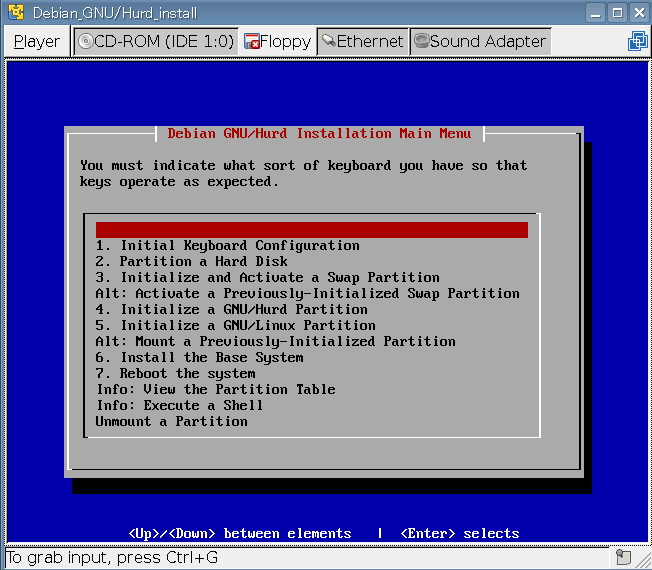
\includegraphics[width=1\hsize]{image200805/hurd0.png}
\end{getsureiupdate}
%===========================================================%

%===========================================================%
\begin{getsureiupdate}{月例 Nexenta Operating System}{上川 純一}
\index{Nexenta}
2008年4月号でインストールしてみた Nexenta Core Platform 1.0 で今月も何か
操作してみます。まず、ホストOSとのデータの交換の方法を確立してみます。

% まず、気が向いたので、kvm で起動してみます。グラフィック機能が超絶に遅い
% のと、ネットワークの接続ができなかった以外は高速に起動しているようです。
% kqemuで稼働させると数分かかるのに比べると高速です。

仮想マシン内部を快適に利用するために、まずSSH接続経由でのファイルシステムを共有をしてみ
 ましょう。
まず、ゲストOSの22番ポートをホストOSの2299番ポートとしてゲストOSを起動し
 てみました。
こうするとssh で localhostの2299番ポートにアクセスして
 ゲストOSにログインできます。

\begin{commandline}
dancer@host$ qemu -hda nexenta.cow -m 512 -redir tcp:2299::22 &
dancer@host$ ssh localhost -p 2299 
Password: 
Last login: Wed Apr 30 05:02:35 2008 from 10.0.2.2
dancer@vm1:~$ 
\end{commandline}

この状態でsshfs を利用するとゲストOSのパスをマウントして見ることができます。ホストOS
からゲストOSの/export/home/dancer にシームレスにアクセスすることができま
す。

\begin{commandline}
dancer@host$ sshfs localhost:  ./nexenta/  -p2299
Password: 
dancer@host$ ls -la nexenta/
合計 36
drwxr-xr-x 1 dancer uucp      9 2008-04-15 23:53 .
drwxr-xr-x 5 dancer dancer 4096 2008-04-30 14:05 ..
-rw------- 1 dancer uucp   1130 2008-04-23 13:05 .bash_history
-rw-r--r-- 1 dancer uucp    220 2008-03-19 18:07 .bash_logout
[以下略]
\end{commandline}

nexenta では各種ファイルを staffグループ (gid=10)が所有し、それがちょうど
Debian では uucpグループ (gid=10) が所有しているように見えています。
\begin{commandline}
dancer@vm1:~$ id dancer 
uid=1000(dancer) gid=10(staff) groups=10(staff)
\end{commandline}
\end{getsureiupdate}
%===========================================================%

\clearpage

\printindex
\clearpage 

メモ欄

\hrule{}

\clearpage 

メモ欄

\hrule{}

\cleartooddpage

\vspace*{15cm}
\hrule
\vspace{2mm}

\includegraphics[width=2cm]{image200502/openlogo-nd.eps}
\noindent \Large \bf Debian 勉強会資料\\ \\
\noindent \normalfont \debmtgyear{}年\debmtgmonth{}月\debmtgdate{}日 \hspace{5mm}  初版第1刷発行\\
\noindent \normalfont 東京エリア Debian 勉強会 (編集・印刷・発行)\\
\hrule


\end{document}

